% Created 2020-10-07 qua 14:53
% Intended LaTeX compiler: pdflatex
\documentclass[11pt]{article}
\usepackage[utf8]{inputenc}
\usepackage[T1]{fontenc}
\usepackage{graphicx}
\usepackage{grffile}
\usepackage{longtable}
\usepackage{wrapfig}
\usepackage{rotating}
\usepackage[normalem]{ulem}
\usepackage{amsmath}
\usepackage{textcomp}
\usepackage{amssymb}
\usepackage{capt-of}
\usepackage{hyperref}
\usepackage{minted}
\usepackage[hyperref, x11names]{xcolor}
\hypersetup{colorlinks = true, urlcolor = SteelBlue4, linkcolor = black}
\usepackage[brazilian]{babel}
\usepackage{geometry}
\geometry{verbose,a4paper,left=2cm,top=2cm,right=3cm,bottom=3cm}
\author{Lourenço Bogo - 11208005}
\date{\today}
\title{Arquitetura de Computadores - Lista 2}
\hypersetup{
 pdfauthor={Lourenço Bogo - 11208005},
 pdftitle={Arquitetura de Computadores - Lista 2},
 pdfkeywords={},
 pdfsubject={},
 pdfcreator={Emacs 27.1 (Org mode 9.3.7)}, 
 pdflang={Brazilian}}
\begin{document}

\maketitle

\section{Questão 1}
\label{sec:org06ba399}
\begin{center}
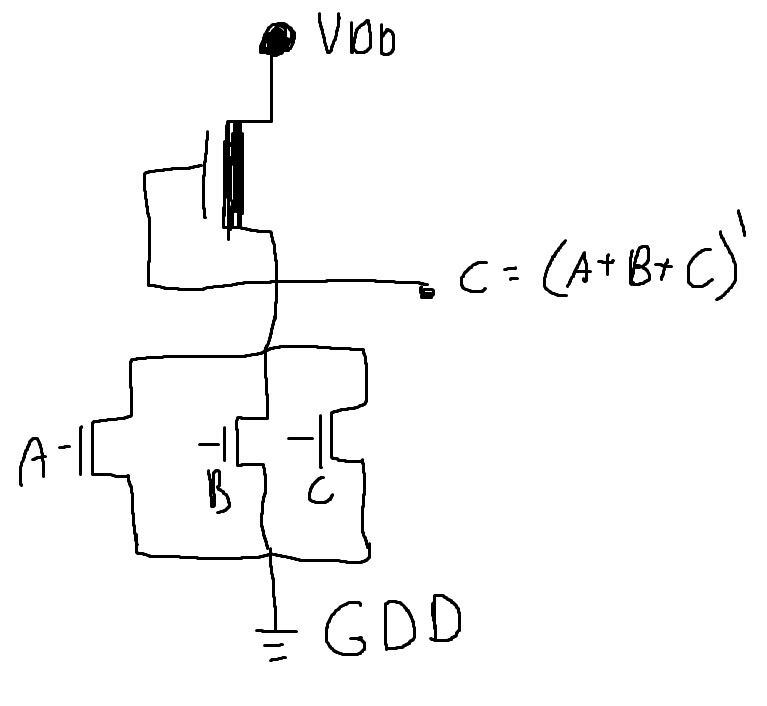
\includegraphics[width=.9\linewidth]{tripleNor.jpg}
\end{center}
\begin{center}
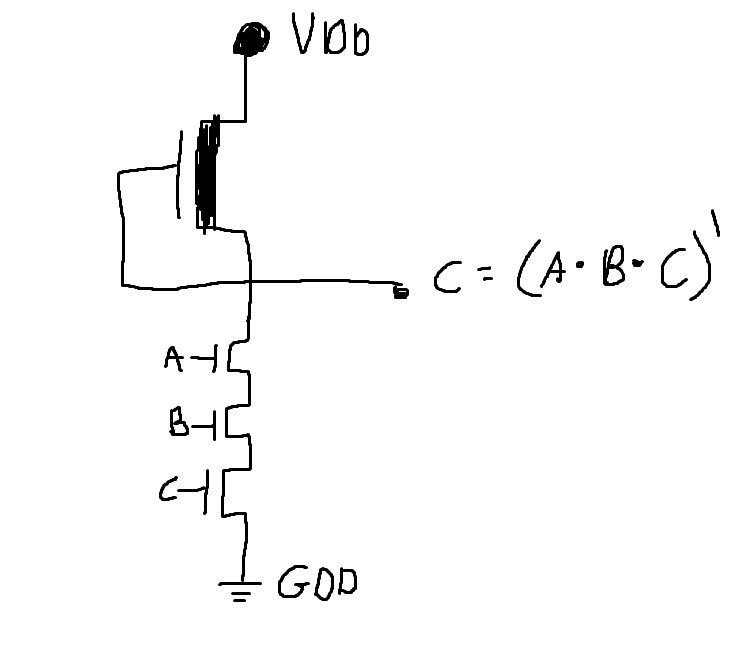
\includegraphics[width=.9\linewidth]{tripleNand.jpg}
\end{center}
\section{Questão 2}
\label{sec:orge36777e}
A alternativa correta é a letra (b): \(r_{ef} = \alpha\frac{L}{W}\).
\section{Questão 3}
\label{sec:orgdac0190}
A alternativa correta é a (b), CMOS.
\section{Questão 4}
\label{sec:org9547be1}
\begin{center}
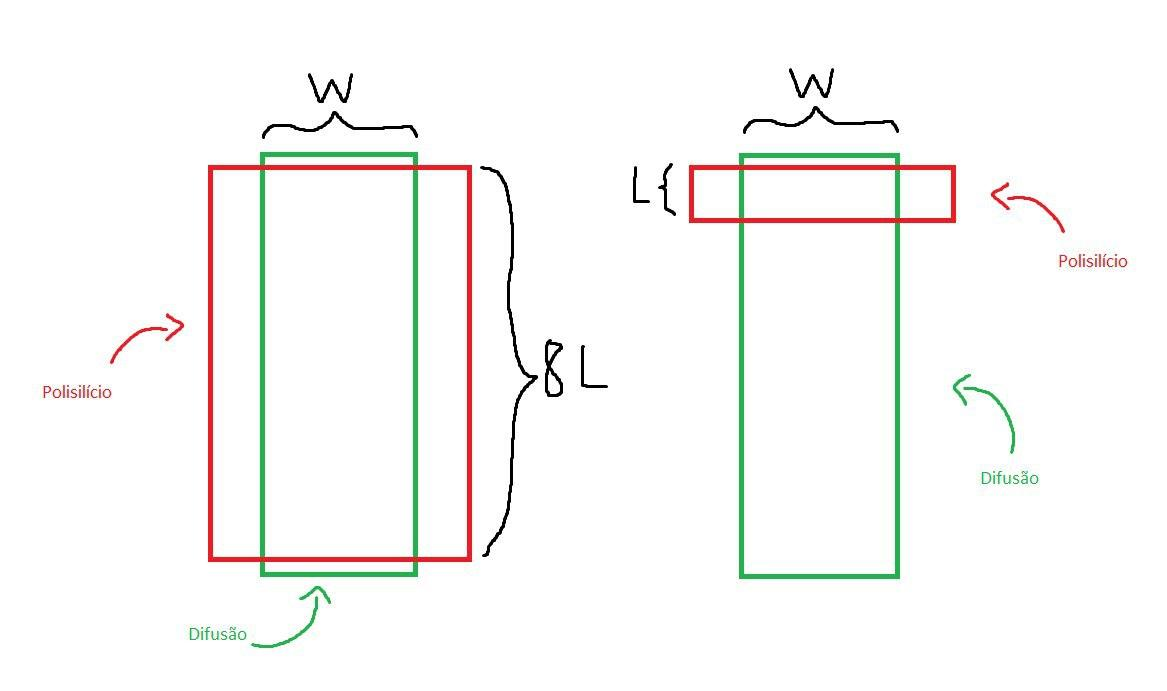
\includegraphics[width=.9\linewidth]{transistors.jpg}
\end{center}
\end{document}